\documentclass[8pt]{beamer}
%epackage[french]{babel}
\usepackage[latin1]{inputenc}
\usepackage{times}
\usepackage{wasysym}
\usepackage[T1]{fontenc}


\definecolor{mongris}{gray}{0.8}           % definition couleur grise
\newcommand{\dd}{\footnotesize $\Diamond$}

\newcommand{\HH}{ \vspace{0.5pt}\hrule}
\newcommand{\round}[1]{\lceil #1 \rfloor}  % notation arrondi
\def\eme{$^{\textrm{{\`e}me}}$}                  % i {\`e}me
\def\num{n^{\circ}}                        % numero
\def\Num{N^{\circ}}                        % Numero
\def\sinc{\mathrm{sinc}}                   % sinus cardinal
\def\ere{$^{\textrm{{\`e}re}}$}                % {\`e}re
\def\er{$^{\textrm{{e}r}}$}                % {\`e}re
\def\eg{\emph{e.g.} }                      % e.g.
\def\ie{\emph{i.e.} }                      % i.e.
\def\etc{\emph{etc}}                       % etc
\def\cm{\,cm}                              % cm
\def\met{\,m}                              % m
\def\mm{\,mm}                              % mm
\def\deg{$^\circ$}                         % degres
\def\ud{\mathrm{d}}                        % pour dx dy ...


\def \R {{\Bbb R}}
\def \I {{\Bbb I}}
\def \H{{\Bbb H}}
\def \F {{\Bbb F}}
\def \S {{\Bbb S}}
\def \B {{\Bbb B}}
\def \Z {{\mathbb Z}}
\def \G {{\mathbb G}}
\def \L {{\mathcal{L}}}
\def \C {{\mathcal C}}
\def \P {{\mathcal P}}
\def \Q {{\mathcal Q}} 
\def \E{{\mathcal E}}
\def \D{{\mathcal D}}
\definecolor{mybluecolor}{RGB}{116,121,149}

\newcommand{\darky}[1]{{\usebeamercolor[fg]{block title example} #1}}
\newcommand{\myblue}[1]{{\color{mybluecolor}\aut{[#1]}}}

\newcommand{\ball}  {\ensuremath{B}}
\newcommand{\AMDR}{\operatorname{AMD}}
\newcommand{\AMD}{\operatorname{AMD}}

\newcommand{\MAset}{\ensuremath{\mathrm{A\!M}} }
\newcommand{\MAsetg}{\ensuremath{\MAset^g } }

\def \PS {{\aut{Planar-4-3-SAT}}}
\def \R {{\Bbb R}}
\def \I {{\Bbb I}}
\def \F {{\Bbb F}}
\def \S {{\Bbb S}}
\def \Z {{\mathbb Z}}
\def \L {{\mathcal{L}}}
\def \C {{\mathcal C}}
\def \P {{\mathcal P}}
\def \Q {{\mathcal Q}} 
\def \E{{\mathcal E}}
\def \D{{\mathcal D}}
\def \BD {{\bar{\mathcal{D}}}}
\def \etal {{\it et al.~}}
\def\arc{\mbox{arc}}
\definecolor{mongris}{gray}{0.8}          
\newcommand{\fup}[1]{\uparrow#1\uparrow}
\newcommand{\fdown}[1]{\downarrow#1\downarrow}
\newcommand{\sI}[1]{\overline{\tt #1}}
\newcommand{\iI}[1]{\underline{\tt #1}}
\newcommand{\e}[5]{#1 & #2 & #3 & #4 & #5 \\}
\newcommand{\eh}[5]{\text{#1} & \text{#2} &  \text{#3} &  \text{#4} & \text{#5}\\} 

\usepackage{beamerthemeliris2}
\useoutertheme{smoothbars}

\title[DGtal]{DGtal: Digital  Geometry Tools and Algorithms Library}
\subtitle{\url{http://liris.cnrs.fr/dgtal}}

\author{}
%\author[DGtal~~~~~~~~~~~~~~~~~~~~~~~~~~David Coeurjolly]{David Coeurjolly}


 \newcommand{\fod}[2]{\multicolumn{2}{p{3.5cm}}{\emph{#1}\dotfill} &
      \multicolumn{2}{p{9cm}}{#2}\\}
    \newcommand{\fodt}[4]{\emph{#1} & {\footnotesize \textsl{#2}} & #3 & \small #4\\}
    % \newenvironment{ta}{\begin{tabular}{p{3.5cm}p{9cm}}}{\end{tabular}\\}
    \newenvironment{ta}{\begin{tabular}{crll}}{\end{tabular}\\}
    % \vfill


\newcommand{\aut}[1]{{\sc #1}}             % auteur en small capsu


%\institute%[XXX]
%{%
%
%  {\bf Laboratoire d'InfoRmatique en Image et Syst�mes d'information} \\
%  { \scriptsize{
%  LIRIS UMR 5205 CNRS/INSA de Lyon/Universit� Claude Bernard Lyon 1/Universit� Lumi�%re Lyon 2/Ecole Centrale de Lyon\\
%  INSA de Lyon, b�timent J. Verne\\
%  20, Avenue Albert Einstein - 69622 Villeurbanne cedex\\
%  \url{http://liris.cnrs.fr}}
%  }
%}



\graphicspath{{./Figures/}, {./../images/},{./Fig/}, {./ICPR2010/},{./Antoine/images/}; {./Images/}}


\begin{document}

\small








\begin{frame}[plain]
  \titlepage
\end{frame}



\begin{frame}
  \frametitle{Table of Contents}
  \tableofcontents
\end{frame}


\begin{frame}
\frametitle{Objectifs}

  \begin{block}{Biblioth�que G�om�trie discr�te\HH}
    \begin{itemize}
    \item faciliter l'appropriation de nos outils pour un n�ophyte
      (nouveau doctorant, chercheur d'une autre discipline, ...)
    \item tester rapidement une nouvelle id�e, permettre une meilleure
      comparaison d'un nouvel outil par rapport � l'existant
    \item faciliter la construction de d�monstrateurs (statiques, en
      ligne, ...)
    \item diffuser nos r�sultats de recherche � d'autres domaines
      \item mettre en place un projet f�d�rateur
\item \ldots
    \end{itemize}
  \end{block}
 

  \begin{block}{Qui ?\HH}
    \begin{itemize}
    \item LIRIS      
    \item LAMA (Chamb�ry)
    \item Gipsa-lab (Grenoble)
    \item LORIA (Nancy)
    \item GREYC (Caen)
    \end{itemize}
  \end{block}
\end{frame}

\begin{frame}
  \frametitle{Objectifs (bis)}

  
  \begin{block}{Pourquoi faire ?\HH}
    \begin{itemize}
    \item D�finir des objets discrets en dimension arbitraire
    \item Proposer des algorithmes d'analyse geom. et topo
    \item D�finir des m�canismes d'I/O et de visualisation
    \end{itemize}
  \end{block}
\end{frame}





\section{Structure}



\begin{frame}
  \frametitle{Sch�ma de structuration}
\small
    \begin{exampleblock}{}
    \centering  Noyau de base
    \end{exampleblock}
    \begin{columns}
      \column{5.5cm}


     \begin{block}{Types et structures de donn�es de base\HH}
      \begin{itemize}
      \item Espace discret, points, vecteurs, alg�bre lin�aire
      \item Infrastructure logicielle : m�canisme de trace, de
        validation de concepts, ...
      \end{itemize}
     \end{block}


      \column{5.5cm}

     \begin{block}{Repr�sentation des images\HH}
      \begin{itemize}
      \item M�canisme de \emph{Container} g�n�rique
      \item Structures adapt�es pour de gros volumes (hashtree,...) 
      \end{itemize}
     \end{block}
      
    \end{columns}



    \begin{exampleblock}{}
    \centering  Modules de base       
    \end{exampleblock}
    \begin{columns}
      \column{5cm}
   \begin{block}{Module topologique\HH}       
      \begin{itemize}
      \item Topologie digitale : ensembles, connexit�, bords,
        compos. connexes
      \item Topologie discr�te : mod�le cellulaire, contours,
        mod�le de repr�sentation de r�gions (Carte Topo/Combi)
      \item Calculs d'invariants n-D
      \end{itemize}
    \end{block}


      \column{5cm}
    \begin{block}{Module g�om�trique\HH}       
      \begin{itemize}
      
      \item Primitives g�om�triques (d�finition, reconnaissance,...) 
      \item Analyse contour : decomposition en primitives,
        estimateurs g�om�triques, ...
      \item Analyse volumique : transformation en distance, axe
        m�dian, ...
      \end{itemize}
    \end{block}
      
    \end{columns}
\end{frame}
\begin{frame}
  \frametitle{Sch�ma de structuration (bis)}


    \begin{exampleblock}{}
   \centering Autres modules ou modules avec d�pendences externes  
    \centering       
    \end{exampleblock}
    \begin{columns}
      \column{5cm}
     \begin{block}{Modules sp�cifiques orient�s projet\HH}
      \begin{itemize}
      \item ANR Geodib (g�om�trie sur objets bruit�s)     
      \end{itemize}
     \end{block}
     \begin{block}{Backends\HH}
      \begin{itemize}
      \item  Kiteware's VTK/ITK
      \item  VIGRA
      \item ... 
      \end{itemize}
     \end{block}
    \column{5cm}

     \begin{block}{Entr�es/sorties\HH} 
      \begin{itemize}
      \item Visualisation vectorielle 2D (svg, xfig, eps)
      \item import/export  diff�rents formats d'image
      \item serialisation,...        
      \end{itemize}
     \end{block}
        \begin{block}{Visualisation/Interfaces\HH} 
      \begin{itemize}
      \item Interface utilisateur
      \item Services web       
      \item ... 
      \end{itemize}
     \end{block}
      
    \end{columns}
\end{frame}



\section{Design et infrastructure}


\begin{frame}
  \frametitle{M�thodologie}

  \begin{block}{Design\HH}
    \begin{itemize}
    \item C++
    \item Prog. g�n�rique
    \item Concepts et mod�les de concept
      \item LGPL ( ou \emph{GPL with restrictions})
    \end{itemize}
  \end{block}


  \begin{block}{Infrastructure\HH}
    \begin{itemize}
    \item  \url{http://liris.cnrs.fr/dgtal}
    \item Tests unitaires
    \item cmake/ctest/cdash
    \item Mailing lists
    \item Doxygen
    \item Tickets trac 
    \item multi-plateforme
    \end{itemize}
  \end{block}

\end{frame}



\section{Exemples}


\begin{frame}
 \frametitle{DGtal v0.2}

 \small
 \begin{exampleblock}{}
   \centering  Noyau de base
 \end{exampleblock}
 \begin{columns}
   \column{5.5cm}
   
   
   \begin{block}{Types et structures de donn�es de base\HH}
     Espace discret, points, vecteurs (nD)
     
     trace, concepts
   \end{block}
   
   
   \column{5.5cm}
   
   \begin{block}{Repr�sentation des images\HH}
     Image container by : STL Vectors, STL Map, Hashtree 
   \end{block}
    \end{columns}

 
 \begin{center}
   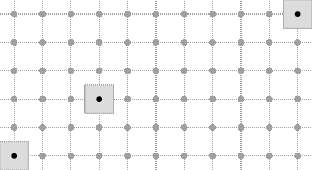
\includegraphics[width=3.5cm]{dgtalboard-1-points.png}~~~~~~~~~~~~~~~~ 
   \includegraphics[width=3cm]{hashtree}
 \end{center}
\end{frame}


\begin{frame}
  \frametitle{DGtal v0.2}
  
 \begin{exampleblock}{}
   \centering  Modules de base       
 \end{exampleblock}
 \begin{columns}
   \column{5cm}
   \begin{block}{Module topologique\HH}       
     \begin{itemize}
     \item Topologie digitale : ensembles, connexit�, bords,
       compos. connexes
     \item Points simples
     \end{itemize}
   \end{block}
   
   
   \column{5cm}
   \begin{block}{Module g�om�trique\HH}       
     \begin{itemize}
      
     \item Primitives g�om�triques : DSS (8,4, O'Rourke)
     \item Analyse contour : GreedyDecomposition
     \item Analyse volumique : DT (n-D optimale)
     \end{itemize}
   \end{block}
   
 \end{columns}
 

 \begin{center}
   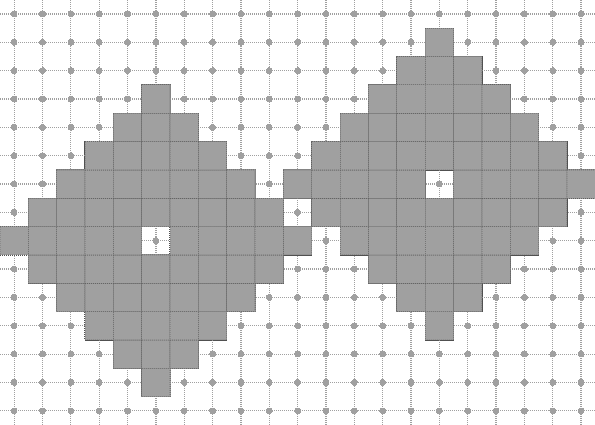
\includegraphics[width=2.5cm]{dgtalboard-2-sets-1.png}~~~~ 
   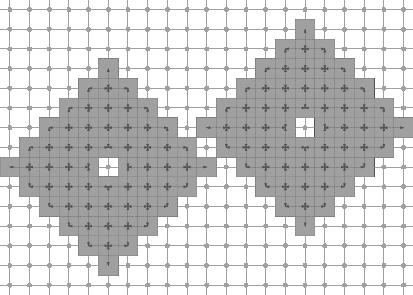
\includegraphics[width=2.5cm]{dgtalboard-2-sets-2.png}~~~~
   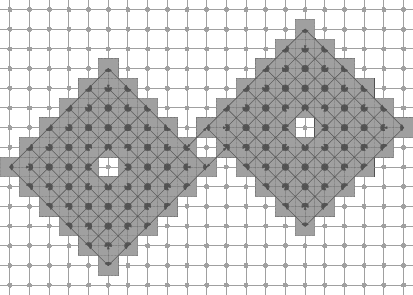
\includegraphics[width=2.5cm]{dgtalboard-2-sets-3.png}\\
   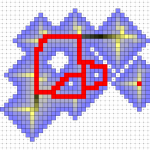
\includegraphics[width=1.7cm]{shape-thinning-4-8-150x150.png}~~~~
   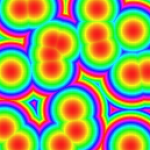
\includegraphics[width=1.7cm]{image-postDT-border-150x150.png}~~~~
   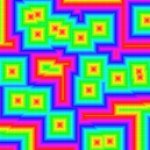
\includegraphics[width=1.7cm]{image-DT-linfty-150x150.png}~~~~
   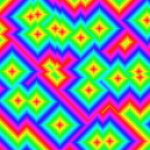
\includegraphics[width=1.7cm]{image-DT-l1-150x150.png}~~~~
   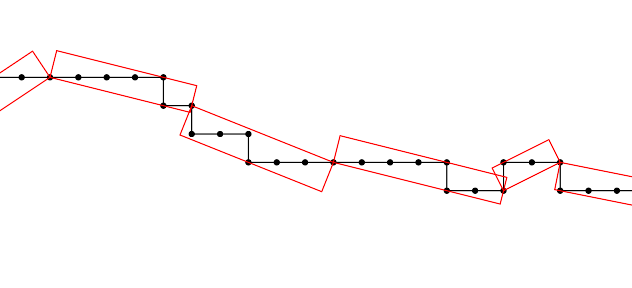
\includegraphics[width=3cm]{segmentation}~~~~
 \end{center}
\end{frame}

\begin{frame}
  \frametitle{DGtal v0.2}
 
 \begin{exampleblock}{}  
   \centering Autres modules      
 \end{exampleblock}
 
 \begin{block}{Entr�es/sorties\HH} 
   \begin{itemize}
   \item 2D: pnm, raw, + beaucoup formats (si ImageMagick install�)
   \item 3D: raw, Vol
   \item nD: raw + serialisation avec boost        
   \end{itemize}
 \end{block}
 

 \begin{block}{Visualisation 2D\HH} 
   \begin{itemize}
   \item DGtalBoard: export SVG, FIG, EPS des objets g�om�triques de
     DGtal (2D)
   \end{itemize}
 \end{block}
\end{frame}

\begin{frame}


exemples...

\begin{itemize}
\item digitalset + board (dgtal-2-sets-*.cpp)
\item DSS reco/decomp
\item distancetransform2D
\end{itemize}
\end{frame}





\section{Conclusion et Milestones}

\begin{frame}
\frametitle{Conclusion}



\begin{block}{Points positifs\HH}
  
  \begin{itemize}
  \item Librairie multi-site
  \item Design g�n�rique, extensible, multi-plateforme
  \item Infrastructure et algorithmes de base performants
  \item M�canisme de visualisation vectorielle 2D  pratique
  \end{itemize}
\end{block}


\begin{exampleblock}{Perspective\HH}
  
  \begin{itemize}
  \item Int�grer de nouveaux sites/d�veloppeurs
  \item Int�grer de nouveaux algorithmes
  \item Construire une documentation orient�e utilisateurs
  \item Poursuivre la construction de ``shortcuts''
  \item Cr�er des d�monstrateurs 
  \end{itemize}
\end{exampleblock}

\begin{alertblock}{Nos besoins\HH}
  \begin{itemize}
  \item D�veloppeurs (accompagnement projets tutor�s)
  \item Relecteurs/r�dacteurs documentation
\item Utilisateurs (retours d'exp�rience rapport de bugs, \ldots) 
  \end{itemize}
\end{alertblock}

\end{frame}

\begin{frame}
\frametitle{Versions futures}

0.3
\begin{itemize}
\item Analyse volum�trique en distance compl�te (RDT, MA)
\item Espace de Khalimsky (mod�le inter-pixel) et operateurs de bord
\item Couverture tangentielle et estimateurs g�om�triques 2D
\item M�canisme de visualisation vectorielle 3D en flux (DGtalBoard3D)
\end{itemize}

0.4
\begin{itemize}
\item Conteneurs d'image avanc�s (tuil�s, backends VTK-ITK,...)
\item Mod�le topologique de partitions (ex. carte combinatoire)
\item Plus de primitives g�om�triques
\item Analyse surfacique en dimension 3 et plus
\end{itemize}

mais tout d�pend de vous...

\end{frame}



\begin{frame}
  \Large
  \begin{center}
    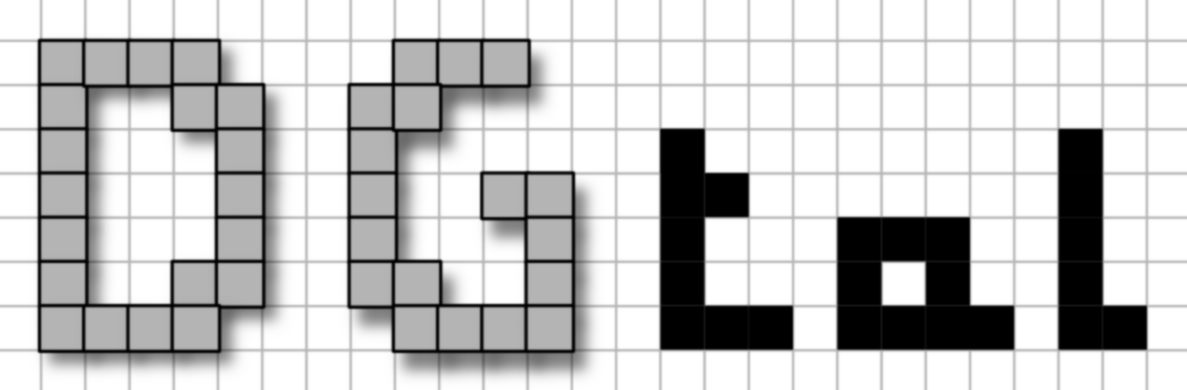
\includegraphics[width=7cm]{logo_DGtal.png} \\~ ~  \\	
    \url{http://liris.cnrs.fr/dgtal}\\~ ~  \\
    \url{dgtal-users@lists.gforge.liris.cnrs.fr}\\
    \url{dgtal-devel@lists.gforge.liris.cnrs.fr}\\
 ~\\
\alert{R�union DGtal : mardi 4 janvier, LIRIS Lyon} 
  \end{center}
\end{frame}




\end{document}



